\chapter{BACKGROUND KNOWLEDGE AND RELATED WORK}
In this chapter, I will introduce the background knowledge of symbolic execution and the related work of my research.
\section{What is Symbolic Execution?}

Symbolic Execution is one of the program analysis techniques whose ultimate goal is to systematically cover all the feasible paths by solving the paths' constraints by using an SMT (Satisfiability Modulo Theory). In order to get the idea of what symbolic execution really is, I will use Snippet \ref{simple_program} as an example to explain the detail of symbolic execution.
\pagebreak
\begin{spacing}{1}
{
\begin{lstlisting}[frame=shadowbox, caption={A Simple Program},label={simple_program}]
int x = 0, y = 0, z = 0;
if (a) {
    x = -2;
}
if (b < 5) {
    if (!a && c) {
        y = 1;
    }
    z = 2;
}
assert(x+y+z != 3)
\end{lstlisting}
}
\end{spacing}

In static analysis, the value of \texttt{x}, \texttt{y} and \texttt{z} will be assigned a variable, then walk through the program to see what part of the code is covered. Then reassign values to \texttt{x}, \texttt{y}, and \texttt{z} and repeat this step until all the possible paths are covered. Apparently, this method is a very low-efficiency method because there is no guarantee that every execution will have a new path be covered. 

Unlike static analysis, symbolic execution is way more efficient. In symbolic execution, no values will be assigned to \texttt{x}, \texttt{y}, and \texttt{z}. Instead, the variables \texttt{x}, \texttt{y}, and \texttt{z} are treated as ``symbol.'' When the execution hit line 2, two constraints will be added. They are \texttt{a == 1} and \texttt{a != 1} representing the \texttt{true} and \texttt{false} of the if-statement respectively. These constraints will be added to two buckets. Each bucket is representing a possible path of this program. Then the engine will continue executing. Once it hits line 5, like the if-statement in line2, two constraints will be produced and added to the buckets. And finally, connecting all the constraints in each bucket with the \texttt{AND} logical operator, an assignment for that path is generated.

\begin{figure}[h]%This [h] tells LaTeX to try to put the picture here.
                 %Without it, it will go to the top of the next page.
\begin{center}
{\mbox{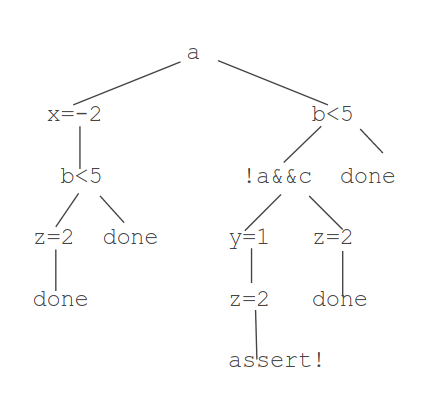
\includegraphics[height=200pt]{figures/path_tree.png}}}
\end{center}
\caption{\label{path_tree}Path Conditions}
\end{figure}

Figure \ref{path_tree} is a tree of path condition of the Snippet \ref{simple_program}. Each of the nodes is a line of code. If a tree node has two children, it means the there is a possible path at that node. Also, the left child representing the \texttt{true} path and the right child representing the \texttt{false} path. To activate the left most path, the testcase should fulfill the constraints of \texttt{(a == 1 AND b < 5)}. To activate the second from the left path, the testcase should fulfill the constraints of \texttt{(a == 1 AND b >= 5)}. To assert, the constraints is \texttt{(a != 1 AND b < 5 AND c == 1)}. The constrains for the rest of two paths is \texttt{(a != 1 AND b < 5 AND c != 1)} and \texttt{(a != 1 AND b >= 5)} respectively.

Comparing static analysis and symbolic execution, the main difference is that symbolic execution get the assignment according to the path it explored, and static analysis gets the assignment before exploring the path. As we can see, there are five possible paths in the program. Therefore, five testcases will be generated to cover all the paths after the symbolic execution process. But for static analysis, probably more than five testcases will be generated to cover all of the feasible paths.

\section{KLEE}

\begin{figure}[h]
\begin{center}
{\mbox{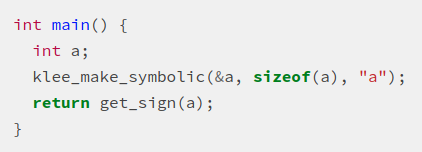
\includegraphics[height=100pt]{figures/make_symbolic.png}}}    
\end{center}
\caption{\label{make_symbolic}Make Input As Symbolic}
\end{figure}

KLEE is a symbolic execution tool that can generate testcases that achieve high coverage on a variety of complex and environmentally-intensive programs automatically \cite{Cadar:2008:KUA:1855741.1855756}. Using the GNU \texttt{COREUTILS} as a benchmark, they covered 90\% of the code on average for all 89 utilities in the package. KLEE can only test the programs that are written in C/C++ and have the source code available. First, a function \texttt{klee\_make\_symbolic} need to be added to the code to mark the input as symbol. Figure \ref{make_symbolic} demonstrates how to make the input symbolic. Then compile the code into LLVM bytecode. The reason for doing so is because KLEE simulates the system environment to handle environmentally-intensive programs. KLEE will execute every line of bytecode to maintain the stack, heap, and etc. for the environment. 

To understand how KLEE works, a critical structure that KLEE implemented need to be introduced. It is \texttt{ExecutionState}. Snippet \ref{execution_state} shows the detail of \texttt{ExecutionState}. \texttt{pc} is the pointer to an instruction to be executed after the current instruction, \texttt{prevPC} is the pointer to the instruction which is currently executed, \texttt{stack} representing the current instruction stream, and \texttt{constraints} collects the constraints so far. Each \texttt{ExecutionState} is representing a valid path. KLEE define a set of operations for each of LLVM instructions. Modifying the data in \texttt{ExecutionState} is completed in those operations. Everytime KLEE hit an if-statement/while-loop/switch-statement or any other instructions that can possibly have a new path; it checks the feasibility of the instruction. If the path is feasible, KLEE will make a copy of the current \texttt{ExecutionState}, and added positive constraints and negative constraints to current \texttt{ExecutionState} and the duplicate. KLEE called this operation \texttt{fork}. After the \texttt{fork} operation complete, KLEE will assign new \texttt{pc} to the current \texttt{ExecutionState} and its copy based on their constraints. Then both of the current \texttt{ExecutionState} and its copy will be put back to the pool and waiting for next round of execution.

Talking at a high level, KLEE completes the analysis task in the following manner. 
\begin{enumerate}
    \item Select one \texttt{ExecutionState} from the pool.
    \item Execute the instruction that \texttt{prevPC} pointed to.
    \item Update the \texttt{ExecutionState} pool.
    \item Repeat step 1.
\end{enumerate}
Snippet \ref{main_logic} indicate this logic. \texttt{states} is the pool of \texttt{ExecutionState}, \texttt{searcher} is responsible for selecting state to execute from \texttt{states}. By default, KLEE will randomly select one \texttt{ExecutionState} from the pool, but it can be depth-first search or a breadth-first search as user's preference.

\begin{spacing}{1}
{
\begin{lstlisting}[frame=shadowbox, caption={ExecutionState},label={execution_state}]
class ExecutionState{
...
KInstIterator pc;
KInstIterator prevPC;
stack_ty stack;
...
ConstraintManager constraints;
...
}
\end{lstlisting}
}
\end{spacing}
\clearpage
\begin{spacing}{1}
{
\begin{lstlisting}[frame=shadowbox, caption={KLEE's Main Logic},label={main_logic}]
while (!states.empty() && !haltExecution) {
    ExecutionState &state = searcher->selectState();
    KInstruction *ki = state.pc;
    ...
    executeInstruction(state, ki);
    ...
    updateStates(&state);
}
\end{lstlisting}
}
\end{spacing}
While the \texttt{ExecutionState} reaches the end or \texttt{pc} points to an invalid address, KLEE will generate a  testcase for that \texttt{ExecutionState} using the solver. The solver consumes the \texttt{constraints} of the \texttt{ExecutionState} and generate a testcase. After receiving the testcase from the solver. The \texttt{ExecutionState} object will be deleted.

\section{Solver}

By default, KLEE uses STP \cite{Ganesh:2007:DPB:1770351.1770421} as the internal solver, but Z3 \cite{DeMoura:2008:ZES:1792734.1792766} can be an option. In general, STP solver emerges as a winner over Z3. By benchmarking \text{[}, \texttt{base64}, \texttt{chmod}, \texttt{comm}, \texttt{csplit}, \texttt{dircolors}, \texttt{echo}, \texttt{env}, \texttt{factor}, \texttt{join}, \texttt{ln} and \texttt{mkfifio}, STP consumes 1,713s to complete, and Z3 takes 3609s \cite{multi-solver-support}. Although KLEE has already got a robust solver, they still have a lot of optimization on the solver side to help the solver run faster. KLEE developed two optimization method on the solver side -- Independent Constraint and Cache. Figure \ref{klee_optimization} shows they process of optimization developed by KLEE.

A query is consist of constraints. Among those constraints, some of them are related, and some of them are not. What KLEE does is they separate the query into little pieces. Each of the pieces contains a set of constraints that have no relation with other constraints. Chopping the query into smaller pieces can not only help the solver to obtain the result faster but also benefits the Cache optimization method as well.

Look up cache before throwing the query to the solver one the useful optimization at the solver side. KLEE maintain a \texttt{Map} in the engine. Using the constraint itself as the key and the counterexample that the solver generates as the value. Before asking solver for the counterexample, KLEE will first check if there is a solved one previously. The idea of this method is query \texttt{Map} is in constant time. Since the \texttt{Map} is maintained in the RAM, ideally, the look up speed should be way more faster than asking solver to generate a counterexample especially when the query is very complicate.

\begin{figure}[h]%This [h] tells LaTeX to try to put the picture here.
                 %Without it, it will go to the top of the next page.
\begin{center}
{\mbox{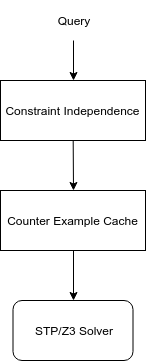
\includegraphics[height=250pt]{figures/klee_optimization.png}}}
\end{center}
\caption{\label{klee_optimization}KLEE's Optimization Method}
\end{figure}

\section{KQuery}

KQuery is a textual representation of the constraint expressions and queries \cite{KQuery}. Currently, KQuery is able to represent a quantifier-free formulas over bitvectors and arrays. It is designed to be easy read and write. Like many other programming languages require variables to be declared before using, bitvectors and arrays need to be declare before querying. A valid query should have the array declaration part and a query command part. Figure \ref{kquery_declaration} shows the syntax of the KQuery declaration. Figure \ref{kquery_query} shows the syntax of a valid query command.

\begin{figure}[h]%This [h] tells LaTeX to try to put the picture here.
                 %Without it, it will go to the top of the next page.
\begin{center}
{\mbox{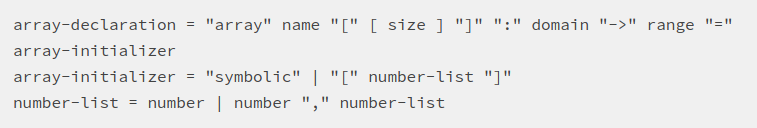
\includegraphics[height=70pt]{figures/kquery_declaration.png}}}
\end{center}
\caption{\label{kquery_declaration}KQuery's Declaration Syntax}
\end{figure}

\begin{figure}[h]%This [h] tells LaTeX to try to put the picture here.
                 %Without it, it will go to the top of the next page.
\begin{center}
{\mbox{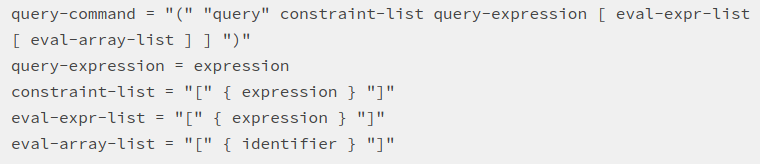
\includegraphics[height=90pt]{figures/query_command.png}}}
\end{center}
\caption{\label{kquery_query}KQuery's Query Command Syntax}
\end{figure}

Combine both the declaration part and the query part can construct a valid query command in the format of KQuery. Snippet \ref{kquery} is a valid query in KQuery format. Translating this query command back to plain English, it is ``Having an array of size 10. The value at the index of 0 is Equal to 77''. For this query command, the solver should return ``\texttt{M000000000}". Note, since the constraint does not have any restriction of other values, the solver will put 0 on those indices by default.

\begin{spacing}{1}
{
\begin{lstlisting}[frame=shadowbox, caption={KQuery},label={kquery}]
array foo[10]: w32 -> w8 = symbolic
(query [(Eq 77 (Read W8 0 foo))] false [] [foo])
\end{lstlisting}
}
\end{spacing}

Not limited to the comparisons, the expression also supports arithmetic operations, bitwise operations. Figure \ref{arithmetic_operations} shows the syntax of arithmetic operations. Figure \ref{bitwise_operations} shows the syntax of bitwise operations. Figure \ref{comparisons} shows the syntax of the comparisons.

\begin{figure}[h]%This [h] tells LaTeX to try to put the picture here.
                 %Without it, it will go to the top of the next page.
\begin{center}
{\mbox{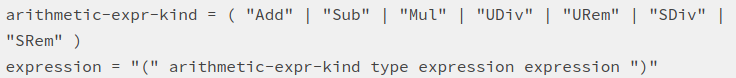
\includegraphics[height=45pt]{figures/arithmetic.png}}}
\end{center}
\caption{\label{arithmetic_operations}KQuery's Arithmetic Operation Syntax}
\end{figure}

\begin{figure}[h]%This [h] tells LaTeX to try to put the picture here.
                 %Without it, it will go to the top of the next page.
\begin{center}
{\mbox{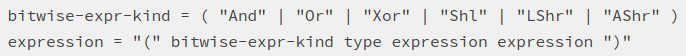
\includegraphics[height=35pt]{figures/bitwise.png}}}
\end{center}
\caption{\label{bitwise_operations}KQuery's Bitwise Operation Syntax}
\end{figure}

\begin{figure}[h]%This [h] tells LaTeX to try to put the picture here.
                 %Without it, it will go to the top of the next page.
\begin{center}
{\mbox{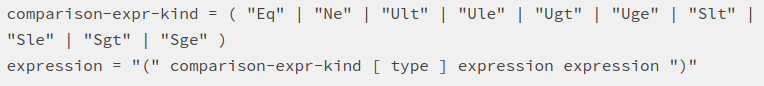
\includegraphics[height=50pt]{figures/comparisons.png}}}
\end{center}
\caption{\label{comparisons}KQuery's Comparisons Syntax}
\end{figure}

The meaning of the expression kinds in arithmetic operations are defined as below:\\
\texttt{Add}: add operation\\
\texttt{Sub}: subtract operation\\
\texttt{Mul}: multiply operation\\
\texttt{UDiv}: truncated unsigned division. Undefined if divisor is 0.\\
\texttt{URem}: Unsigned remainder. Undefined if divisor is 0.\\
\texttt{SDiv}: Signed division. Undefined if divisor is 0.\\
\texttt{SRem}: Signed remainder. Undefined if divisor is 0. Sign of the remainder is the same as that of the dividend.\\

The meaning of the expression kinds in bitwise operations are defined as below:\\
\texttt{And}: and operation.\\
\texttt{Or}: or operation.\\
\texttt{Xor}: xor operation.\\
\texttt{Shl}: logical shift left. For example, \texttt{(Shl TYPE X Y)} means moves each bit of \texttt{X} to the left by \texttt{Y} positions. The \texttt{Y} right-most bits of \texttt{X} are replaced with zero, and the left-most bits discarded.\\
\texttt{LShr}: logical shift right.\\
\texttt{AShr}: arithmetic shift right. Behaves as \texttt{LShr} except that left-most bit of \texttt{X} copy the initial left-most bit of \texttt{X}.\\

The meaning of the expression kinds of comparisons are defined as below:\\
\texttt{Eq}: equal.\\
\texttt{Ne}: not equal.\\
\texttt{Ult}: unsigned less than.\\
\texttt{Ule}: unsigned less or equal to.\\
\texttt{Ugt}: unsigned greater than.\\
\texttt{Uge}: unsigned greater or equal to.\\
\texttt{Slt}: signed less than.\\
\texttt{Sle}: signed less or equal to.\\
\texttt{Sgt}: signed greater than.\\
\texttt{Sge}: signed greater or equal to.\\
\section{Related Work}

The goal of this thesis is to address the the most significant issue of symbolic execution. A lot of people have done some fantasitc work to solve this problem before. I was inspired by one of the previous projects. In that project, the researchers modified KLEE's own data structure to serialize a query in order to send out to the remote solver \cite{Rakadjiev:2015:PSS:2847598.2847727}. This method has fast query transfer speed. However, it limits the symbolic execution engine to be KLEE. It can't support multiple different symbolic execution tools working at the same time. To avoid this disadvantages, I decided to send out a query in KQuery format. Since KQuery is a textual representation of the queries and constraints, technically, all of the constraints can be represented in the format of KQuery. This method allows another engine to use the remote solver by sacrificing some of the query transfer time.

In my remote solver, I also adopt KLEE's optimization method -- Constraint Independence and Caching. The main difference is that KLEE uses cache for the same program because KLEE is a synchronous engine. The solver is built-in in the engine. Once KLEE finishes the analysis task, the solver will be terminated and cache will be cleared. My solver is a remote solver, and it will not be terminated. Therefore, the cache will always exist. All of the queries can share the same cache map. I argue that this method can reduce the number of counterexample that generates by the solver. 